\documentclass[11pt]{article}

\usepackage[margin=1in]{geometry}
\usepackage{times}
\usepackage{setspace}
\usepackage{amsmath}
\usepackage{hyperref}
\usepackage{tikz}
\usetikzlibrary{positioning, arrows.meta, shapes}

\setstretch{1.15}

\title{\textbf{Context-Aware Synonym Replacement Using Learned Representations}}
\author{Sebastian Lopez \and Diego Bonilla \\ Texas Tech University}
\date{CS4391 -- Homework 1 \\ Spring 2026}

\begin{document}
\maketitle

\section{Introduction}

This homework investigates whether pretrained semantic representations can support context-aware synonym replacement without relying on large language models, masked language models, or lexical databases. The objective is not fluent generation, but understanding how embeddings encode meaning and where they fail—particularly in metaphorical or poetic language.

We design a controlled pipeline that replaces a selected word in each sentence while attempting to preserve sentence-level meaning using embedding-based similarity.

\section{System Overview}

The system follows a modular pipeline:

\begin{itemize}
    \item Sentence segmentation
    \item Target word selection (last non-stopword)
    \item Synonym candidate generation using word embeddings
    \item Heuristic grammatical filtering
    \item Context-based scoring using sentence embeddings
\end{itemize}

A replacement is accepted only if semantic similarity with the original sentence exceeds a predefined threshold.

\section{Model Selection}

\subsection{Word Embeddings}

Candidate synonyms are generated using the \texttt{glove-wiki-gigaword-100} pretrained embeddings. This model offers broad semantic coverage and efficient nearest-neighbor retrieval, making it suitable for exploratory experimentation.

\subsection{Sentence Embeddings}

Contextual compatibility is evaluated using the \texttt{all-MiniLM-L6-v2} Sentence-BERT model. This lightweight transformer produces sentence-level embeddings that allow cosine similarity comparisons between original and modified sentences.

\section{Experimental Results}

\subsection{Filtering Effects}

Early experiments with minimal filtering produced frequent grammatical errors, such as plural mismatches and noun–adjective shifts. Adding lightweight grammatical constraints significantly reduced these failures while preserving semantic flexibility.

\subsection{Threshold Sensitivity}

We tested similarity thresholds from 0.70 to 0.90. Lower thresholds allowed more substitutions but often damaged metaphorical meaning, while higher thresholds became overly restrictive. A threshold of \textbf{0.86} provided the best balance and was used for final results.

\section{Examples}

\subsection{Literal Replacement}

\textbf{Original:} ``Two roads diverged in a yellow wood.'' \\
\textbf{Modified:} ``Two roads diverged in a yellow timber.''

The substitution preserves meaning and structure, confirmed by a high sentence similarity score.

\subsection{Metaphorical Preservation}

\textbf{Original:} ``Hope is the thing with feathers.'' \\
\textbf{Modified:} (unchanged)

No candidate exceeded the similarity threshold, correctly preserving the metaphor.

\section{Failure Analysis}

Several systematic limitations remain:

\begin{itemize}
    \item \textbf{Polysemy:} Embeddings conflate multiple word senses (e.g., \textit{players}).
    \item \textbf{Metaphor Loss:} Semantic similarity reflects association, not figurative intent.
    \item \textbf{Grammatical Drift:} Sentence embeddings tolerate singular/plural changes.
    \item \textbf{Stylistic Insensitivity:} Phonetic and rhetorical effects are ignored.
\end{itemize}

These failures stem from fundamental properties of distributional semantics rather than implementation choices.

\section{Use of AI in This Homework}

AI tools were used as interactive collaborators to clarify concepts, accelerate experimentation, diagnose failures, and assist with report structuring. All architectural decisions and interpretations were critically evaluated by the authors.

\subsection{AI-Assisted Workflow}

Figure~\ref{fig:ai-workflow} illustrates the collaborative development process.

\begin{figure}[h]
\centering
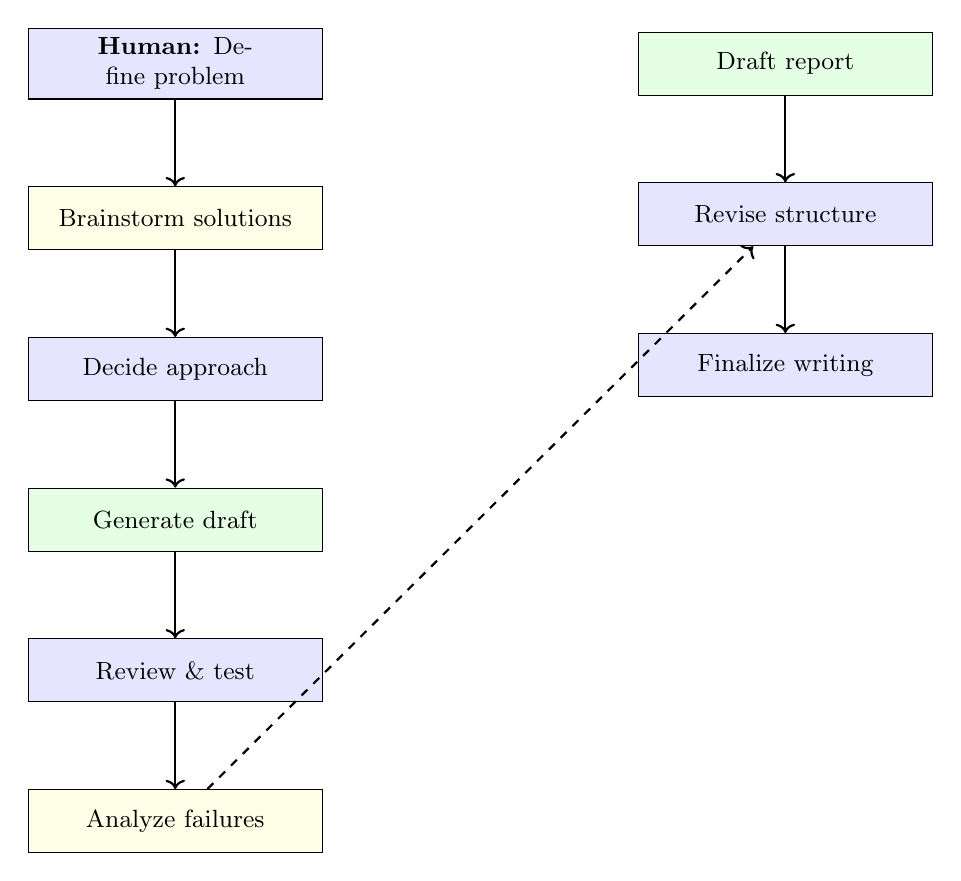
\begin{tikzpicture}[
    node distance=1.1cm,
    box/.style={rectangle, draw, text width=3.5cm, align=center, minimum height=0.8cm, font=\small},
    human/.style={box, fill=blue!10},
    ai/.style={box, fill=green!10},
    collab/.style={box, fill=yellow!10},
    arrow/.style={->, thick}
]

\node[human] (problem) {\textbf{Human:} Define problem};
\node[collab] (brainstorm) [below=of problem] {Brainstorm solutions};
\node[human] (decide) [below=of brainstorm] {Decide approach};
\node[ai] (code) [below=of decide] {Generate draft};
\node[human] (review) [below=of code] {Review \& test};
\node[collab] (debug) [below=of review] {Analyze failures};

\node[ai] (template) [right=4cm of problem] {Draft report};
\node[human] (revise) [below=of template] {Revise structure};
\node[human] (final) [below=of revise] {Finalize writing};

\draw[arrow] (problem) -- (brainstorm);
\draw[arrow] (brainstorm) -- (decide);
\draw[arrow] (decide) -- (code);
\draw[arrow] (code) -- (review);
\draw[arrow] (review) -- (debug);

\draw[arrow] (template) -- (revise);
\draw[arrow] (revise) -- (final);

\draw[arrow, dashed] (debug) -- (revise);

\end{tikzpicture}
\caption{AI-assisted workflow for system development and report writing.}
\label{fig:ai-workflow}
\end{figure}

\section{Conclusion}

This work demonstrates that embedding-based similarity enables effective literal synonym replacement but fails systematically on metaphor, polysemy, and stylistic language. These limitations highlight the gap between distributional semantics and human language understanding and motivate more expressive models for context-sensitive text manipulation.

\end{document}


